% This document must be compiled with LuaLaTeX
\documentclass[12pt,article]{memoir}

\usepackage[letterpaper, portrait, margin=1in]{geometry}	% Standard page setup
\usepackage[USenglish]{babel}								% English typsetting conventions
\usepackage{fancyhdr}										% Headers and footers
\usepackage{graphicx}										% Additional graphics options
\usepackage{xcolor}											% Better colors
\usepackage{xpatch}											% Better macro patches
\usepackage{hyperref}										% Hyperlinks
\usepackage{fontspec}										% Custom fonts
\usepackage{tikz}											% Graphics creation
\usepackage{float}											% Figure positioning
\usepackage{tabu}											% Better tables
\usepackage[style=ieee, backend=biber]{biblatex}			% Bibliography
\usepackage[font={small,it}]{caption}						% Italic captions
\setsansfont{NeueHaasUnicaPro}
\usetikzlibrary{calc}
\usepackage[yyyymmdd]{datetime} % change date format to yyyy/mm/dd to fit ISO8601

\renewcommand{\familydefault}{\sfdefault} % set font
\renewcommand{\dateseparator}{--} % change date-seperators to - to fit ISO8601

\renewcommand\contentsname{Table of Contents}

\chapterstyle{section}
\renewcommand*{\chapnumfont}{\normalfont\HUGE\bfseries\sffamily}
\renewcommand*{\chaptitlefont}{\normalfont\HUGE\bfseries\sffamily}

\makeatletter 
% define macro for itemcode
\newcommand\itemcode[1]{\renewcommand\@itemcode{#1}}
\newcommand\@itemcode{}

% define macro for rev number
\newcommand\revnumber[1]{\renewcommand\@revnumber{#1}}
\newcommand\@revnumber{}
\makeatother

\definecolor{orbitOrange}{RGB}{250,62,0} % the ORBiT orange

\setlrmarginsandblock{2.5cm}{2.5cm}{*}
\setulmarginsandblock{2.5cm}{*}{1}
\checkandfixthelayout 

\setlength{\beforechapskip}{0cm} % reduce chapter spacing

\hypersetup{
    colorlinks,
    citecolor=black,
    filecolor=black,
    linkcolor=black,
    urlcolor=black
}

% Background swoosh
\newcommand\OrbitBackground[1]{% For a logo drawn with TikZ
	\begin{tikzpicture}[remember picture,overlay] % draw background
	\coordinate (bl) at (current page.south west);
	\coordinate (r) at (current page.east);
	\coordinate (A) at ($(bl)+(0,3cm)$);
	\coordinate (B) at ($(r)+(0,-2cm)$);
	\coordinate (C) at (current page.south east);
	\coordinate (ctrlNode) at ($(current page.south) + (0cm,1cm)$);
	\coordinate (ctrlNode2) at ($(current page.south east) + (-1cm,1cm)$);
	\fill[orbitOrange, fill opacity={#1}]
	(A) .. controls (ctrlNode) and (ctrlNode2) .. (B) -- (C) -- (bl);
	\node [white] at ($(C) + (-3cm,1cm)$) {2015-\the\year \ ORBiT@SU};
	\end{tikzpicture}
}

% Bibliography database
\addbibresource{DR00001.bib}

%**********************************************************************
%Document titles etc. defined here: (replace [] as well)
\title{OA-II Backplane Bus System Design}
\author{Jinzhi Cai}
\itemcode{DR00001}
\revnumber{A03}
\date{\today}
%end of document titles etc.
%**********************************************************************
% set header style
\makeatletter
\pagestyle{fancy}
{
	\fancyheadoffset{0cm}

	\lhead{\@title \ - \@itemcode}
	\rhead{Page: \thepage }
	%\chead{\leftmark} % section name
}
\makeatother

\cfoot{\OrbitBackground{0.2}}

\begin{document}
	
\OrbitBackground{1}

\makeatletter

\includegraphics[width=\textwidth]{../Templates/logo.jpg}\\[4ex]
\begin{center}
	\bfseries \fontsize{50}{50}\selectfont  \@title \\[2ex]
	\LARGE  \@itemcode
\end{center}
\vfill
\begin{flushright}
	\LARGE Rev: \@revnumber\\
	\large \@author\\
	\large \@date\\[18ex]
\end{flushright}
\makeatother
\thispagestyle{empty}
\newpage

\tableofcontents*
\thispagestyle{fancy}
\newpage

\tableofcontents*
\newpage


%**********************************************************************
% Everything after this is the main document. Edit below this line,

\chapter{Introduction}
\section{Scope}
This document analyzes the requirements for OA-II VEH system data transmission, and current bus technologies in the field. It outlines a system design to fulfill the needs of OA-II VEH system.
\section{Purpose}
The goal for the OA-II VEH backplane bus system is to construct a fast, versatile, compact, and highly robust backplane data transmission system.
\section{Revision History}
\begin{table}[H]
	\centering
	\begin{tabu}{r || c | c | c }
		Rev\# & Editor & Delta & Date\\ \hline
		A01 & Jinzhi Cai & Initialize & 2019-7-19\\\hline
		A02 & Jinzhi Cai & Add detail Ethernet & 2019-7-22\\
		A03 & Gabriel Smolnycki & Edits for clarity & 2019-08-17
	\end{tabu}
	\caption{Summary of Revision History}
	\label{tab:rev}
\end{table}
\newpage

\chapter{Bus System Requirements}
\section{Hardware Requirements}
\begin{description}
	\item[Backplane Bus]The bus needs to support interchangeable modules.
	\item[Vibration Resistant]The bus needs provide resistance high shock and vibration.
	\item[Size]The bus needs to fit inside the rocket payload section.
	\item[Topology]The hardware implementation cannot be location dependent.
\end{description}
\section{Software Requirements}
\begin{description}
	\item[Point to Point \& Broadcast]The bus needs to support broadcasting data.
	\item[Bandwidth]The bus needs to support the max bandwidth given.
	\item[Topology]The bus topology should be software defined and reconfigurable.
	\item[Priority]The bus needs to support message priority levels, including real-time communication.
	\item[Multiple Speeds]The bus needs to allow both high and low speed devices.
\end{description}

\section{Bandwidth Calculation}
\subsection{Low Speed Payload}
Low speed payloads generate data at a minimum of 10kHz/16bit.
\begin{itemize}
\item 4 high pressure sensors for propulsion system
\item 2 low pressure sensors for pitot tube
\item 4 high temperature sensors for propulsion system
\item 4 low temperature sensors for electronics
\item 4 low temperature sensors for batteries
\item 2 low temperature sensor for ambient
\end{itemize}
\begin{equation}
	4+2+4+4+4+2=20 channels
\end{equation}
\begin{equation}
	16 bits (b) = 2 bytes (B)
\end{equation}
\begin{equation}
	10kHz \times 2B =20kB/s
\end{equation}
\begin{equation}
	20kB/s \times 20 = 400kB/s
\end{equation}

\subsection{High Speed Payload}
\begin{itemize}
\item 9 axis IMU
\item GNSS system
\item 4x 1080p@60Hz cameras
\end{itemize}

For a 9 axis IMU at 10kHz/16bit per axis:
\begin{equation}
	9 \times 10kHz \times 2B = 180kB/s
\end{equation}

For a typical GNSS module running at 10Hz\footnote{Not including a safety factor}:
\begin{itemize}
	\item UTC launch time - 4 bytes
	\item Latitude - 4 bytes
	\item Longitude - 4 bytes
	\item Altitude - 4 bytes
	\item Direction + Ground speed - 4 bytes
\end{itemize}
\begin{equation}
	4B \times 5 = 20B
\end{equation}
\begin{equation}
	10Hz \times 20B =200B/s
\end{equation}

For cameras, assume a compressed bitrate of 8Mb/s\footnote{High bitrate is necessary for high vibration environment}:
\begin{equation}
	8Mb/s = 1MB/s
\end{equation}
\begin{equation}
	1MB/s \times 4 = 4MB/s
\end{equation}

\subsection {Total bandwidth}
\begin{table}[H]
	\centering
	\begin{tabu}{r || c | c | c }
		Device & Number & Bandwidth per Device & Total Bandwidth\\ \hline
		High Pressure Sensors & 4 & 20KB/s & 80KB/s\\
		Low Pressure sensors & 2 & 20KB/s & 40KB/s\\
		High Temperature Sensors & 4 & 20KB/s & 80KB/s\\
		Low Temperature Sensors & 10 & 20KB/s & 200KB/s\\
		9 axis IMU & 1 & 180KB/s & 180KB/s\\
		GNSS system & 1 & 200B/s & 200KB/s\\
		Cameras & 4 & 1MB/s & 4MB/s
	\end{tabu}
	\caption{Summary of Estimated Bandwidth}
	\label{tab:bandwidth}
\end{table}

Using a factor of safety of 2 to compensate for encoding overhead:
\begin{equation}
	(180kB/s + 4MB/s + 200B/s + 400kB/s) \times 2 \approx 10MB/s
\end{equation}

\newpage

\chapter{Analysis of common bus protocols}
\section{I2C}
I2C is a serial protocol for two-wire interface to connect low-speed devices like microcontrollers, EEPROMs, A/D and D/A converters, I/O interfaces and other similar peripherals in embedded systems. It was invented by Philips and now it is used by almost all major IC manufacturers \cite{blog:I2C}.\par
I2C is a great low speed communication bus, however it does not support hardware priority level and software defined topology.

\section{SPI}
Serial Peripheral Interface (SPI) is an interface bus commonly used to send data between microcontrollers and small peripherals such as shift registers, sensors, and SD cards \cite{blog:SPI}.\par
SPI allows the device to increase its bandwidth by increasing the data clock rate. However, it does not support hardware priority level or software defined topology.

\section{UART}
A universal asynchronous receiver-transmitter is a computer hardware device for asynchronous serial communication in which the data format and transmission speeds are configurable \cite{blog:UART}.\par
UART does not require a clock line to transmit data. It also can use individual bitrates per device. However it is a point to point communication system, so it needs a switch for more than two devices. It also does not support high enough bandwidth to meet the requirements.

\section{CAN}
A Controller Area Network (CAN bus) is a robust vehicle bus standard designed to allow microcontrollers and devices to communicate with each other in applications without a host computer \cite{canbus:CAN}.\par
CANbus has hardware priority level support and works up to 500kbps\footnote{62.5kB/s} bandwidth. It also allows group broadcast as well as point to point communication.

\section{PCIe}
PCI Express, officially abbreviated as PCIe or PCI-e, is a high-speed serial computer expansion bus standard, designed to replace the older PCI, PCI-X and AGP bus standards. It is the common motherboard interface for personal computers' graphics cards, hard drives, SSDs, Wi-Fi and Ethernet hardware connections \cite{MR:PCIe}.\par
PCI Express is a commonly used bus in personal computers. It supports up to 16GT/s\footnote{1.969 GB/s} per lane. However, it mostly uses a tree type topology. As a result, it is difficult to add a second master to the system.

\section{RapidIO}
The RapidIO architecture is a high-performance packet-switched interconnect technology. RapidIO supports messaging, read/write and cache coherency semantics \cite{RapidIO:RapidIO}.\par
RapidIO is a high speed connection that supports up to 5Gbps\footnote{About 625MB/s} per lane. It also supports multi-master structure. Using a RapidIO switch, software defined technology is also possible. However, RapidIO is a new bus technology that is mainly used in DSPs, high speed FPGAs, and SoCs. It require significant hardware resources compared to the other buses.

\section{SpaceWire}
SpaceWire is defined in the European Cooperation for Space Standardization standard ECSS-E-ST-50-12C (replaces ECSS-E50-12A). The SpaceWire standard was authored by Steve Parkes, University of Dundee with contributions from many individuals within the SpaceWire Working Group from European Space Agency (ESA), European Space Industry, Academia and NASA \cite{ESA:SpaceWire}. There is also a successor called SpaceFibre, which allows up to 15 times higher data rates per lane, while maintaining significant compatibility with SpaceWire \cite{ESA:SpaceFibre}.\par
The SpaceWire uses the LVDS voltage standard which is a commonly use voltage standard in FPGAs. The PHY for SpaceWire is relatively simple and does not require significant resources. The newest SpaceWire bus supports speeds of up to 400Mbps per lane\footnote{50MB/s}. 

\section{Interlaken}
Interlaken was invented by Cisco Systems and Cortina Systems in 2006, optimized for high-bandwidth and reliable packet transfers. It builds on the channelization and per channel flow control features of SPI-4.2, while reducing the number of integrated circuit (chip) I/O pins by using high speed SerDes technology \cite{blog:Interlaken}.\par
Interlaken is designed to replace Ethernet. It supports port division and flow control, however the Interlaken PHY is not supported by many FPGAs. This means that it will require an extra PHY chip. It supports similar speeds to RapidIO\footnote{625MB/s}.

\section{Ethernet}
Ethernet is a widely used bus that has many benefits to the data bus system, as its standard is implemented in many devices and drivers, and a router for it is easy to develop. It also can go up to 1Gbps\footnote{125MB/s} with appropriate PCB design. However, it does not have a real time clock as with SpaceWire, and is not as fast as RapidIO or PCIe. Ethernet is also not designed for realtime applications \cite{blog:Ethernet}.

\newpage
\chapter{Recommended System Design}
\section{Bus Structure}
Based on the requirements of the bus, the OA-II Bus System will include two parts: the command bus, which is in charge of the initialization of devices bus and then prioritizes data transmission, and the data bus which is in charge of the transmission of large amounts of data (including telemetry) and of programs. The job for those two buses will be different during each stage\footnote{More detail is included in \textit{ES00007 - OA-II Payload Bus Specifications}}.
\subsection{Initialization}
\begin{description}
	\item[Command Bus] ON
	\item[Data Bus] Configuration
\end{description}
In the initialization stage, OA-II VEH COM MCU will detect all the on board devices and run a self-test ensure all devices are functioning correctly. During this stage, all communication occurs via the command bus, and each device will initialize and configure its data bus interface. Finally, the MCU will send a request on the command bus and receive acknowledgment on the data bus.

\subsection{Pre-launch}
\begin{description}
	\item[Command Bus] ON
	\item[Data Bus] ON
\end{description}
After the initialization stage, the vehicle will enter the pre-launch stage. At this stage, all programs will be loaded onto their respective modules via command bus and wait for an ignition signal for synchronization. All sensors will be running at full speed and deliver data to the MCU to monitor vehicle status via the data bus.

\subsection{During Flight}
\begin{description}
	\item[Command Bus] Standby
	\item[Data Bus] ON
\end{description}
After ignition and during flight, all sensors will be running at full speed and deliver data to the MCU to monitor vehicle status and for recording via the data bus. The command bus will be in standby mode and ready to send an emergency messages.

\subsection{Post-flight}
\begin{description}
	\item[Command Bus] Standby
	\item[Data Bus] OFF
\end{description}
After landing, the MCU will again run a self test on all modules before turning off power. The data bus will be off during the landing process.

\subsection{Emergency Backup}
\subsubsection{Scenario 1 - Command Bus Failure}
When COM FRU detects a command bus failure, it will disable COM MCU control and use the data bus to send out a Failure Alert to all modules. The data bus will only transmit critical data and commands. Other data units will be powered off or save data to their internal storage.
\subsubsection{Scenario 2 - Data Bus Failure}
When COM FRU detects a data bus failure, it will use command bus to communicate with MCU and check the MCU status. The mission will continue and all modules will switch communications to the secondary data bus, running at a lower speed. 

\subsection{Bus Data Summary}
\begin{table}[H]
	\centering
		\begin{tabu}{ c | c | c | c }
		& From: COM & From: TAM & From: PAM \\ \hline
		To: COM & X & Data Bus & Data Bus \\ \hline
		To: TAM & Command Bus/Data Bus & X & Data Bus \\ \hline
		To: PAM & Command Bus & Data Bus & X \\ \hline
		\end{tabu}
	\caption{Communication routes}
	\label{tab:routes}
\end{table}
\begin{table}[H]
	\centering
		\begin{tabu}{ c | c }
		Command Bus & Data Bus\\ \hline
		Mission critical & Not mission critical\\
		Low bitrate data & High bitrate data\\
		Realtime data & Research data\\
		Internal communication & Communication with base station\\
		\end{tabu}
	\caption{Bus Data Catalog}
	\label{tab:busdata}
\end{table}

\newpage

\section{System Redundancy}
The command bus will have two separate and redundant physical buses. The primary and secondary command buses will send the same command at the same time. Each device will receive information from the primary bus, and use the secondary bus for error checking.\par
Each unit will have a two lane connection to each data bus router. Both buses will send and receive the same information. Each device will receive information from the primary bus, and use the secondary bus for error checking.\par
During the Initialization stage, the primary data router will synchronize configuration with the second data routing core. When the configuration is finished, the link will be disabled.
\begin{figure}[H]
\begin{center}
	\centering
	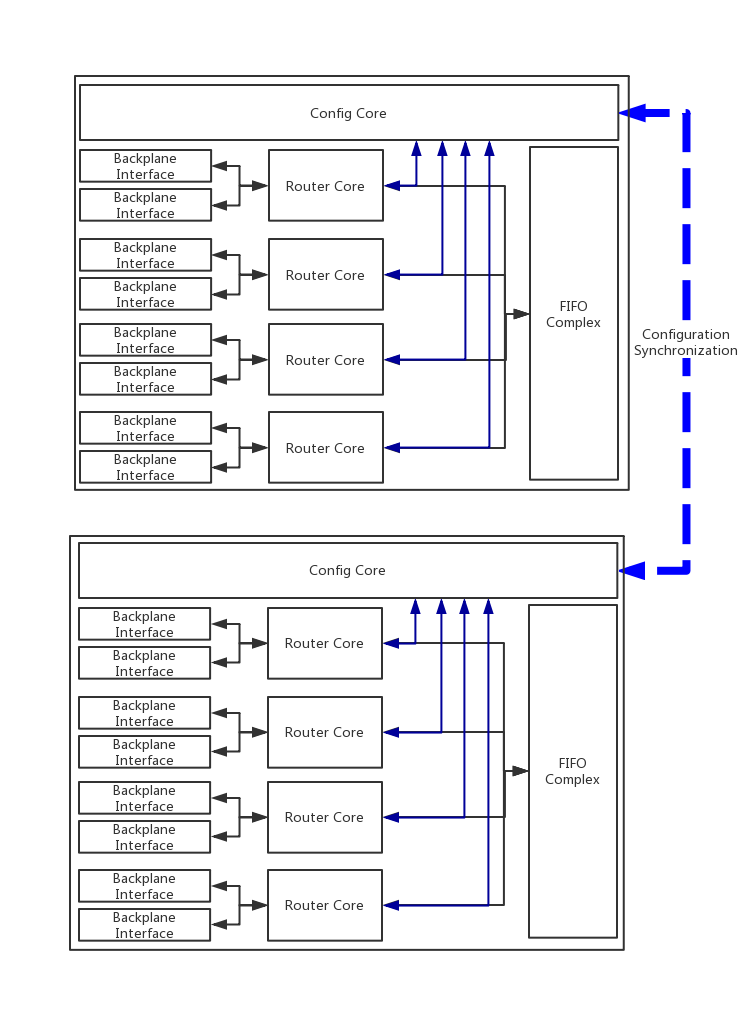
\includegraphics[width=4.0in]{img/DR00001_SpaceWire_2.png}
	\caption{Data Router Structure}
\end{center}
\end{figure}

\newpage

\section{CAN + SpaceWire}
\begin{description}
	\item[Command Bus] CAN
	\item[Data Bus] SpaceWire
\end{description}
In this setup, the command bus uses CAN. It provides prioritized data transmission for small amounts of data transmission, and speeds up to 500kbps, which is enough bandwidth for command data transmission. The data bus uses SpaceWire which provides enough bandwidth for high speed data transmission. It also includes a timestamp feature that will help in sensor fusion. The system is built around two routers, where one is the main router that will be used for primary data transmission and the other is a backup router which can take over in the event the main router fails.
\begin{figure}[H]
	\centering
	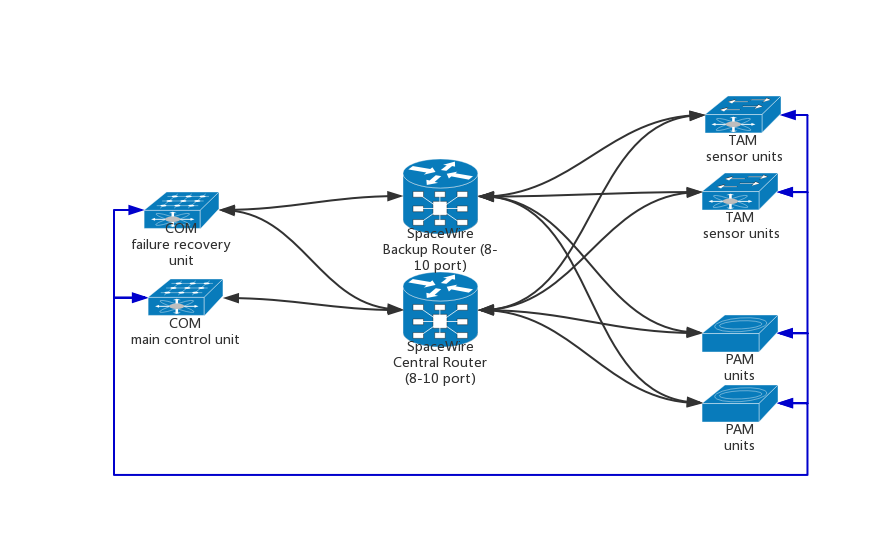
\includegraphics[width=\textwidth]{img/DR00001_SpaceWire_1.png}
	\caption{Recommended Design A}	
\end{figure}

\newpage

\section{CAN + RapidIO}
\begin{description}
	\item[Command Bus] CAN
	\item[Data Bus] RapidIO
\end{description}
In this setup, CAN bus still is the main command bus due to its prioritized data transmission. However, the data bus uses RapidIO, where each lane can carry 10 times data rate compared to SpaceWire. This will handle most future advanced missions without significant hardware upgrades. This will require a separate ASIC for as a RapidIO router. This setup is more difficult to implement, but is a viable upgrade path from a CAN + SpaceWire design.
\begin{figure}[H]
	\centering
	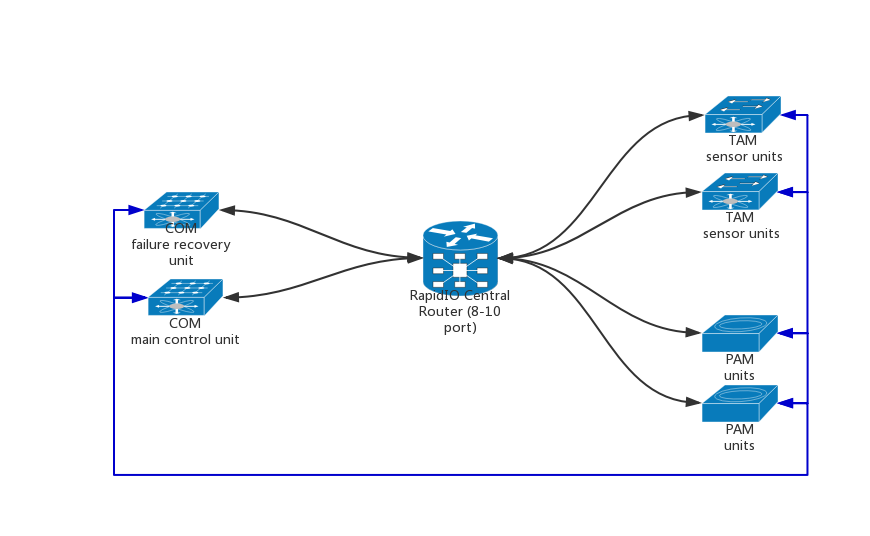
\includegraphics[width=\textwidth]{img/DR00001_RapidIO.png}
	\caption{Recommended Design B}
\end{figure}

\newpage

\chapter{Bibliography}
\printbibliography[heading=none]

\end{document}
